\documentclass{article}

\usepackage{polski}
\usepackage[utf8]{inputenc}
\usepackage[ruled,vlined]{algorithm2e}
\usepackage{indentfirst}
\usepackage{amssymb}

\usepackage{graphicx}
\usepackage{float}
\graphicspath{ {./images/} }

\usepackage[backend=biber]{biblatex}
\addbibresource{bibliography.bib}

\usepackage{amsmath}
\renewcommand{\vec}[1]{\mathbf{#1}}

\title{GA \& DNN}
\author{Jan Sołtysik}


\begin{document}
\maketitle
\tableofcontents


\section{Wstęp}


\section{Wprowadzenie teoretyczne}

\subsection{Algorytm Genetyczny}
Algorytmy genetyczne są to algorytmy poszukiwania zainspirowane mechanizmem doboru naturalnego
oraz dziedziczności. Łączą w sobie ewolucyjną zasadę przeżycia najlepiej przystosowanych 
osobników z systematyczną, choć zrandomizowaną wymianą informacji. W każdym pokoleniu powstaje
nowy zespół sztucznych organizmów, utworzonych z połączenia fragmentów najlepiej przystosowanych
przedstawicieli poprzedniego pokolenia. Oprócz tego sporadycznie wyporóbowuje się nową część 
składową. Element losowości nie oznacza że algorytmy genetyczne sprowadzają się do zwykłego
błądzenia przypadkowego. Dzięki wykorzystaniu przeszłych doświadczeń algorytm określa nowy obszar
poszukiwań o spodziewanej podwyższonej wydajności.
Algorytm genetyczny jest przykładem procedury używającej wyboru losowego jako 
"przewodnika" w wysoce ukierunkowanym poszukiwaniu w zakodowanej przestrzeni rozwiązań
\cite{goldberg}.\\

Poniżej znajduję się podstawowy algorytm genetyczny przedstawiony w postaci
pseudokodu \cite{ams}:\\
\begin{algorithm}[H]
 \SetAlgoLined
 \KwIn{Funkcja oceny $f(\vec{x})$}
 \KwOut{Wektor $\hat{\vec{x}}$ dla którego $f(\hat{\vec{x}})$ jest lokalnym minimum}
 Niech $t = 0$ będzie licznikiem generacji. 
 Wygeneruj $n_x$ - wymiarową populację $\mathcal{C}(0)$, składającą się z n osobników.\\
 \While{Warunek końcowy nie jest prawdziwy}{
	Oblicz przystosowanie, $f(\vec{x}_i(t))$ każdego osobnika $\vec{x}_i(t)$ z populacji.\\
	Zastosuj operatory genetyczne oby stworzyć potomstwo.\\
	Wybierz nową populację. $\mathcal{C}(t + 1)$.\\
	Przejdź do nowej generacji. $t = t + 1$.\\
 }
 \caption{Podstawowy Algorytm genetyczny}
\end{algorithm}

\subsubsection{Podstawowa reprezentacja}
W elementarnym AG osobniki nazywane \textbf{genomami} reprezentujemy za pomocą ciągów bitów.
Poniżej znajduję się przykładowy genom:\\

\begin{figure}[H]
\centering
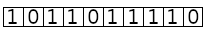
\includegraphics[scale=1.0]{genome.png}
\caption{Przykładowy genom o długości 10.}
\end{figure}

Transformacja naszego problemu do opisu w postaci ciągów binarnych jest często bardzo trudne, a
czasami wręcz niemożliwe. Lecz trud ten jest opłacalny ponieważ dla tak opisanych genomów mamy
zdefiniowane operatory genetyczne których poprawność jest dowiedziona matematyczne. Natomiast w
przypadku użycia innej reprezentacji osobników musimy zdefiniować własne operatory oraz nie mamy
pewności co do ich efektywności.

\subsubsection{Selekcja}
Jest to etap algorytmu w którym wybieramy poszczególne genomy które później zostaną poddane operatorom genetycznym.
Aby opisać ten proces musimy zdefiniować przedstawioną w \textbf{Algorytmie 1} funkcję oceny 
$f$.\\
\textbf{Funkcja oceny/przystosowania} $f$ jest obliczana dla każdego osobnika i pozwala nam
porównać które genomy są najlepiej przystosowane do zadania które optymalizujemy.\\
Najprostszym przykładem będzie zadanie znalezienia maximum funkcji 
$g(x_1, ..., x_n)$ gdzie $n \in \mathbb{N}^{+}$, wtedy funkcja przystosowania
będzie równa wartości funkcji $g$, im większa wartość $g$ tym osobnik jest
lepiej przystosowany.\\\\
Istnieje wiele metod selekcji lecz zdecydowanie najpopularniejszą jest \textbf{metoda ruletki}
w której prawdopodobieństwo $p_i$
wybrania $i$-tego genomu do reprodukcji kolejnego pokolenia jest proporcjonalne do wartości
funkcji przystosowania i jest równe:
\begin{equation}
	p_i = \frac{f_i}{\sum_{j=1}^{N} f_j}
\end{equation}
gdzie:\\
$f_i$ - wartość funkcji oceny dla $i$-tego genomu, $N$ - rozmiar populacji.\\

\subsubsection{Krzyżowanie}
Jednym z dwóch podstawowych operacji wykonywanych w celu stworzenia potomstwa obecnej populacji
jest \textbf{krzyżowanie}, które inspiruję się rozmnażaniem płciowym w biologi
\textbf{[Wikipedia]}.

W literaturze możemy znaleźć wiele rodzai tej operacji, poniżej znajdują się najpopularniejsze
odmiany:
\begin{itemize}
\item \textbf{Krzyżowanie jednopunktowe}:\\
W tej odmianie potomka tworzymy z dwóch wybranych przez selekcję rodziców a następnie 
losujemy punkt $l$ z przedziału $[0, n_x)$. Potomek wartości na pozycjach $[0, l)$
przyjmuje wartości z pierwszego rodzica, natomiast na pozycjach $[l, n_x)$ z drugiego.
\begin{figure}[H]
\centering
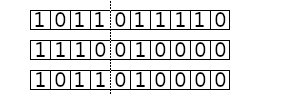
\includegraphics[scale=5.0]{crossover.png}
\caption{Krzyżowanie jednopunktowe, gdzie $n_x = 10$ i $l = 4$.}
\end{figure}

\item \textbf{Krzyżowanie dwupunktowe}:\\
Sposób ten jest zbliżony do opisanego wyżej lecz zamiast jednego punktu losujemy dwa
$l_1, l_2 \in [0, n_x)$, gdzie $l_1 < l_2$. Potomek natomiast przyjmuje wartości z pierwszego
rodzica poza elementami na pozycjach $[l_1, l_2)$ gdzie wstawiamy elementy z drugiego.

\begin{figure}[H]
\centering
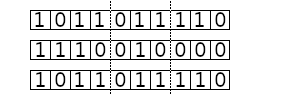
\includegraphics[scale=5.0]{two_crossover.png}
\caption{Krzyżowanie dwupunktowe, gdzie $n_x = 10$, $l_1 = 4$ i $l_2 = 7$.}
\end{figure}

Krzyżowania tego rodzaju można uogólnić na operacje gdzie losujemy k-punktów
a potomek naprzemiennie pobiera wartości z rodziców.\\
\item \textbf{Krzyżowanie równomierne}:\\
Potomek każdy element jest wybierany z obu rodziców z takim równym prawdopodobieństwem.
(Można również wybrać inny stosunek prawdopodobieństw).

\end{itemize}

\subsubsection{Mutacja}
Operator ten w klasycznej wersji algorytmu polega na zamienieniu wartości znajdującej się na 
losowo wybranej pozycji z bardzo małym prawdopodobieństwem $\sigma_m$(np. 0.2\%).
\begin{figure}[H]
\centering
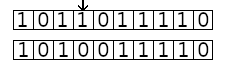
\includegraphics[scale=1.0]{mutation.png}
\caption{Podstawowa mutacja dla genomu o $n_x = 10$ i wylosowanej pozycji 3.}
\end{figure}



\subsection{Sztuczne Sieci Neuronowe}
Podobnie jak dla Algorytmów Genetycznych, inspiracją dla Sztucznych Sieci Neuronowych (SSN) 
byłą biologia a dokładniej budowa neuronów naturalnych znajdujących się w ciele człowieka.
Zostały one wymyślone już w w pierwszej połowie XX wieku, lecz dopiero w ostatnich latach
dzięki rozwojowi technologi oraz dostępności do olbrzymiej ilości danych mogliśmy zacząć używać
ich pełnego potencjału. SSN są przykładem techniki \textbf{uczenia nadzorowanego} tzn.
podczas uczenia sieci podajemy mu dane z znanymi wynikami i poprzez porównywanie wygenerowanych
wyników z rzeczywistymi nasza sieć uczy się generować poprawne wyniki.

\subsubsection{Perceptron}
\textbf{Perceptron} to  najprostsza architektura SSN. Jednostki na wyjściach/wejściach
nazywane są \textbf{neuronami}. Na neuronach wejściowych  podawane są liczby oraz
każde połączenie ma przypisaną,  wagę natomiast wyjście perceptronu jest obliczane przez 
wyliczenie ważoną sumę sygnałów wejściowych:
\begin{equation}
	z = \sum_{i=1}^n w_ix_i = \vec{w}^T\vec{x}
\end{equation}
gdzie:\\
$w_{ij}$ - waga połączenia pomiędzy $i$-tym neuronem wejściowym a $j$-tym wyjściowym,\\
$x_i$ - $i$-ta wartość wejściowa.\\ \\
Następnie wynik otrzymany w (1) jest poddawany \textbf{funkcji skoku}, gdzie najczęściej jest 
ona równa \textbf{funkcji Hraviside'a} lub \textbf{signum} które są równe:
\[
	\text{Heaviside}(z) = \
	\begin{cases}
		0, \: z < 0 \\
		1, \: z \geq 0
	\end{cases} 
	\text{sgn}(z) = \
	\begin{cases}
		-1, \: z < 0 \\
		0, \: z = 0 \\
		1, \: z > 0
	\end{cases} 
\]
Nazywane są one \textbf{funkcjami aktywacji}.\\

\begin{figure}[H]
\centering
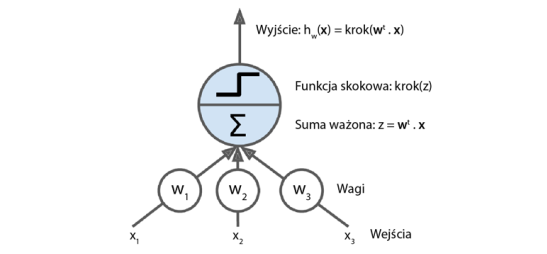
\includegraphics[scale=0.5]{perceptron.png}
\caption{Schemat perceptronu z jednym neuronem wyjściowym i trzema wejściowymi}
\end{figure}

Lecz aby na wyjściu otrzymywać oczekiwane wyniki musimy najpierw perceptron wytrenować. Proces
ten polega na modyfikacji wag na podstawie porównanie wyniku oczekiwanego z wynikiem otrzymanym.
Wagi jest aktualizowana według wzoru:
\begin{equation}
	w_{ij} = w_{ij} + \eta(y_j - \hat{y_j})x_i
\end{equation}
gdzie:\\
$\hat{y_i}$ - otrzymany wynik na $j$-tym wyjściu,\\
$y_j$ - docelowy wynik $j$-tego neuronu,\\
$\eta$ - współczynnik uczenia.
Perceptron jednak nie nadaję się do skomplikowanych zadań ponieważ przez swoją prostą budowę
jest jedynie zdolny do klasyfikowania danych na zabiory,które są liniowo separowalne.

\subsubsection{Wielowarstwoa Sieć Neuronowa}
Ograniczenia perceptronu można wyeliminować tworząc SSN z wielu warstw perceptronów.
SSN tego typu nazywamy \textbf{perceptronem wielowarstwowym}, który jest złożony z 
\textbf{warstwy wejściowej}, co najmniej jednej \textbf{warstwy ukrytej} (jako wejście przyjmują
one wyjście poprzedniej warstwy a ich wyjście propagowane do kolejnej jako wejście) ostatnią
warstwę nazywamy \textbf{warstwą wyjściową}. Dodatkowa w każdej warstwie znajduję się 
\textbf{neuron obciążający} jego zadaniem jest wysyłanie na wejście następnej warstwy 
wartości 1. Ilość neuronów w warstwie wejściowej i wyjściowej jest określana przez
zestaw danych na których sieć ma pracować np. jeśli zadaniem sieci jest rozpoznawanie
ręcznie pisanych cyfr to na wyjściu powinno znaleźć się 10 neuronów a na wejściu każdy neuron
powinien odpowiadać jednemu pikselowi wczytanego obrazu.
SSN która zawiera co najmniej dwie warstwy ukryte nazywamy
\textbf{głęboką siecią neuronową} (GSN).

\begin{figure}[H]
\centering
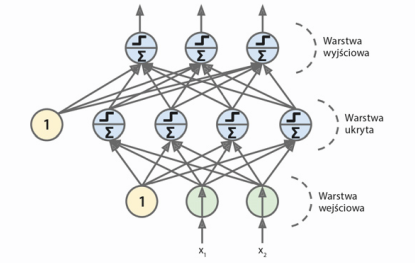
\includegraphics[scale=0.5]{gsn.png}
\caption{Perceptron wielowarstwowy z jedną warstwą ukrytą.}
\end{figure}

Lecz ponieważ nasza sieć składa się z wielu warstw metoda uczenia używana dla pojedynczego
perceptronu nie spiszę się w tym przypadku. Najpopularniejszą metodą uczenia sieci neuronowych 
jest \textbf{wsteczna propagacja} (alternatywnie do uczenia SSN można użyć np. Algorytmów
Genetycznych). Cały proces możemy przedstawić za pomocą kroków:\textbf{[stronka\_z\_ssn]}:

{\LinesNumbered
\begin{algorithm}[H]
 Wybór parametrów sieci (liczba warstw, liczba neuronów w warstwach itd.)\\
 Wagi inicjujemy losowo.\\
 Błąd dla każdego neuronu obliczany jest błąd równy różnicy pomiędzy otrzymanym
 wynikiem $\hat{\vec{y}}$ a wartością oczekiwaną $\vec{y}$.\\
 Błędy propagowane są do poprzednich warstw.\\
 Modyfikacja wag na podstawie wartości błędu.\\
 Powtarzaj od \textbf{3} dla kolejnych wektorów uczących.\\
 Skończ algorytm jeśli przekroczymy ustaloną liczbę epok, lub średni błąd przestanie zauważalnie
 maleć.\\
 \caption{Procedura uczenia wielowarstwowej SSN.}
\end{algorithm}}
Średni błąd może być przestawiony przez wzór:
\begin{equation}
	d = \frac{1}{2}(\hat{\vec{y}} - \vec{y})^2
\end{equation}
Podczas aktualizowania wag wybieramy te wartości dla których średni błąd jest najmniejszy, możemy
je znaleźć np. używając metodę gradientu prostego przy użyciu odwrotnego różniczkowania
automatycznego.

\subsubsection{Funkcje aktywacyjne}
Aby powyższy algorytm przebiegał prawidłowo zamiast funkcji skokowej/signum wprowadzono inne 
funkcje aktywacji, ponieważ funkcje używane w przypadku pojedynczego perceptronu są złożone
jedynie z płaskich segmentów, co uniemożliwia korzystać z gradientu. Poniżej znajdują się 
najczęściej używane \textbf{funkcje aktywacji} w SSN:
\begin{itemize}
\item \textbf{funkcja logistyczna}:\\
W każdym punkcie ma zdefiniowaną pochodną niezerową, dzięki czemu algorytm gradientu prostego
może na każdym etapie uzyskiwać lepsze wyniki. Jest ona używana w warstwie wyjściowej jeśli
zadaniem naszej sieci jest klasyfikacja obiektów na przynależność do dwóch rozłącznych klas.
Dodatkowo jest to funkcja używana przez neurony 
naturalne przez co uważana była za najlepszą funkcję aktywacyjną, lecz jak pokazała praktyka
w przypadku SSN inne funkcje sprawują się lepiej.
\begin{equation}
\sigma(z) = \frac{1}{1 + e^{-z}}
\end{equation}
\item \textbf{funkcja tangensa hiperbolicznego}:\\
Jest S - kształtna, ciągłą i różniczkowalna, podobnie jak funkcja logistyczna, 
ale zakres wartości wynosi $(-1, 1)$ a nie $(0, 1)$.
\begin{equation}
	\tanh(z) = 2\sigma(2z)-1
\end{equation}
\item \textbf{funkcja ReLU}:\\
Jest ciągłą, ale nieróżniczkowalna dla $z = 0$. W praktyce jednak spisuje się znakomicie 
dodatkowo jest bardzo szybko obliczana. Aktualnie jest ona oraz jej odmiany są najczęściej
używanymi funkcjami aktywacji dla warstw ukrytych i wejściowej. 
\begin{equation}
	ReLU(z) = \max(0, z)
\end{equation}
\item \textbf{funkcja softmax}:\\
Używana jest ona w warstwie wyjściowej jeśli nasza sieć ma obliczać
prawdopodobieństwa przynależności otrzymywanych obiektów  do klas 
(jest ich więcej niż 2 i wszystkie prawdopodobieństwa mają się sumować do $1$).
Model najpierw oblicza dla każdej klasy - $k$:
\begin{equation}
	s_k(\vec{x}) = \big(\vec{w}^{(k)}\big)^T\vec{x}
\end{equation}
gdzie: $\vec{w}^{(k)}$ - wyspecjalizowany wektor wag dla klasy $k$.\\
Po wyliczeniu $s_k(\vec{x})$ dla każdej klasy, obliczane jest odpowiednio znormalizowane 
prawdopodobieństwo przynależności danej próbki do klasy $k$:
\begin{equation}
	p_k = \frac{\exp\big(s_k(\vec{x})\big)}{\sum_{i=1}^{K} \exp\big(s_i(\vec{x})\big)}
\end{equation}
gdzie: $K$ - liczba klas.\\ 
Model prognozuję klasę o najwyższym prawdopodobieństwie:
\begin{equation}
	\hat{y} = \underset{k}{\text{argmax}}(p_k)
\end{equation}
\end{itemize}

\begin{figure}[H]
\centering
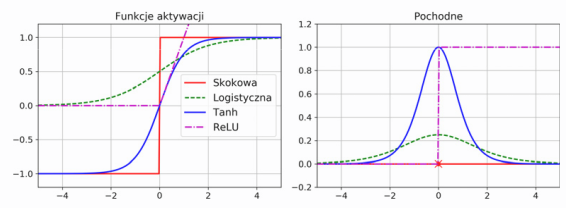
\includegraphics[scale=0.6]{f_a.png}
\caption{Funkcje aktywacyjne i ich pochodne.}
\end{figure}

\subsubsection{Inne rodzaje warstw SSN.}
W SSN oprócz \textbf{warstw gęstych} tzn.
gdzie każdy neuron w $i$-tej warstwie jest połączony z wszystkimi neuronami
znajdującymi się w warstwie nr. $i+1$,
używane są warstwy innych które pomagają siecią
osiągać lepsze wyniki. Oto kilka przykładowych warstw:
\begin{itemize}
\item \textbf{warstwa splotowa}:
Używane są one w zadaniach wizualnych. Neurony w pierwszej warstwie splotowej nie są
połączone z każdym połączone z każdym pikselem obrazu wejściowego, lecz wyłącznie z pikselami
znajdującymi się w ich polu recepcyjnym.

\begin{figure}[H]
\centering
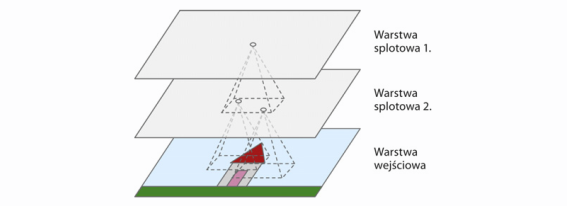
\includegraphics[scale=0.6]{cnn.png}
\caption{Warstwy CNN z prostokątnymi lokalnymi polami recepcyjnymi.}
\end{figure}

Dzięki powyższej strukturze sieć może koncentrować się na ogólnych cechach w pierwszej warstwie
ukrytej, następnie łączyć je w bardziej złożone kształty w kolejnych warstwach. Ogólnie neuron
znajdujący się w $i$-tym wierszu oraz $j$-tej kolumnie danej warstwy jest połączony z wyjściami 
neuronów poprzedniej warstwy zlokalizowanymi w rzędach od $i \cdot s_h$ do 
$i \cdot s_h + f_h-1$  i kolumnach
od $j \cdot s_w $ do $j \cdot s_w + f_w-1$
gdzie: $f_w/f_h$ - szerokość/wysokość pola recepcyjnego, $s_h, s_w$ definiują wartość 
\textbf{kroków} odpowiednio w kolumnach i rzędach. \textbf{Krokiem} nazywamy odległość
pomiędzy dwoma kolejnymi polami recepcyjnymi. Aby uzyskać takie same rozmiary wymiary 
dla każdej warstwy najczęściej dodawane są zera wokół wejść.\\

Wagi neuronu mogą być przedstawione jako niewielki obraz o rozmiarze pola recepcyjnego, tak 
zwane \textbf{filtry}. Przykładowo filtrem może być macierz wypełniona zerami oprócz środkowej
kolumny zawierającej jedynki, neurony posiadające taki filtr będą ignorować wszystkie elementy
oprócz tych które znajdują się w środkowej linii.

\begin{figure}[H]
\centering
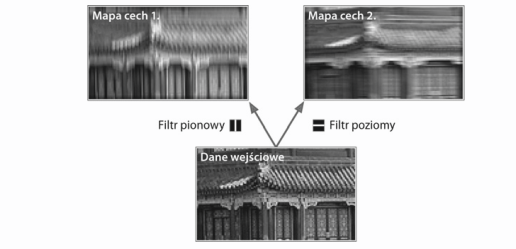
\includegraphics[scale=0.6]{filtr.png}
\caption{Dwie mapy cech otrzymane przy pomocy dwóch różnych filtrów.}
\end{figure}

Warstwa wypełniona neuronami o takim
samym filtrze nazywamy \textbf{mapą cech} która pomaga nam wyszczególnić elementy przypominające
użyty filtr. Warstwa splotowa składa się z kilku map cech o identycznych rozmiarach.
Każda mapa ma swoje wartości parametrów, dzięki czemu stosując przez stosowanie różnych
filtrów warstwa splotowa jest w stanie wykryć wiele cech w dowolnym obszarze obrazu.
Dodatkowo obrazy wejściowe składają się również z kilu warstw, po jednej na każdy kanał
barw. Zazwyczaj są to trzy kanały - czerwony, zielony i niebieski lub jeden dla obrazów
czarno-białych.


\begin{figure}[H]
\centering
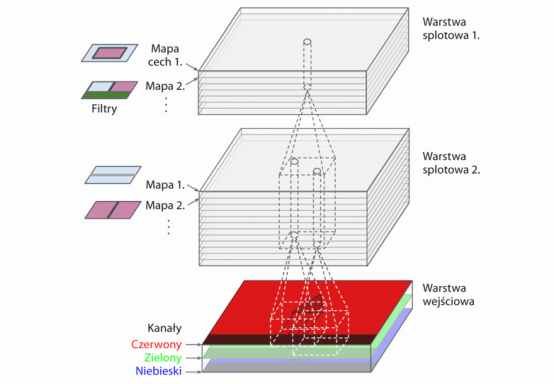
\includegraphics[scale=0.6]{rgb_cnn.png}
\caption{Warstwa splotowa zawierająca wiele cech, oraz zdjęcie z trzema kanałami barw.}
\end{figure}

\item \textbf{warstwa łącząca}:
Jej celem jest zmniejszenie obrazu wejściowego w celu zredukowania obciążenia obliczeniowego,
wykorzystania pamięci i liczby parametrów. Tak samo jak w warstwach splotowych neurony 
łączą się z wyjściami określonej liczby neuronów poprzedniej warstwy, które mieszczą się w
obszarze pola recepcyjnego. Jednakże warstwa ta nie zawiera wag, jej zadaniem jest gromadzenie
danych przy pomocy funkcji agregacyjnej np. maksymalizującej lub uśredniającej.

\begin{figure}[H]
\centering
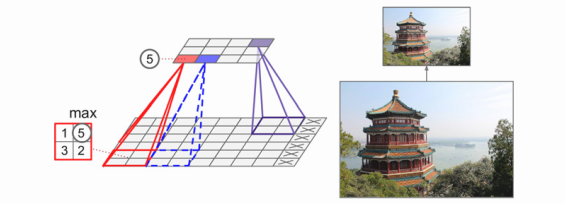
\includegraphics[scale=0.6]{pool.png}
\caption{Maksymalizująca warstwa łącząca, gdzie rozmiar jądra łączącego to 2x2.}
\end{figure}

\item \textbf{warstwa porzucania}:\\
Warstwa ta dla poprzedniej warstwy aplikuję technikę \textbf{porzucania} tzn. że
każdy neuron znajdujący się w tej warstwie w poszczególnym przebiegu może zostać całkowicie
pominięty w procesie uczenia. Szansa na porzucenie jest hiperparametrem i nazywana jest 
\textbf{współczynnikiem porzucenia}.

\begin{figure}[H]
\centering
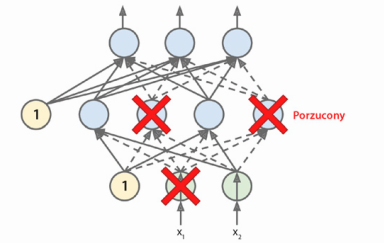
\includegraphics[scale=0.6]{dropout.png}
\caption{Przykład porzucania.}
\end{figure}

\end{itemize}
Istnieje wiele innych rodzai warstw w SSN (np. rekurencyjne) lecz opisałem tyko warstwy
użyte w moim programie. Z tego samego powodu jedyną opisaną przeze mnie architekturą jest
\textbf{jednokierunkowa sieć neuronowa}(sygnał biegnie w jednym kierunku).

\section{Micro - GA dla SSN}
SSN posiadają dużą liczbę hiperparametrów i wpływ każdego z nich na efektywność sieci jest
zależny od wykonywanego zadania, więc jeżeli wybieramy je ręcznie musimy to robić
metodą prób i błędów. Aby użyć AG to tego zadania musimy zmodyfikować jego tradycyjną odmianę.
Ponieważ zależy nam na szybkości wykonywanych obliczeń zastosowana została odmiana 
\textbf{micro-GA} gdzie liczba dozwolonych generacji jest niewielka. Dodatkowo aby przyśpieszyć
działanie algorytmu SSN są trenowane przez ograniczoną liczbę epok tzw. \textbf{uczenie
częściowe}.

\begin{algorithm}[H]
 \SetAlgoLined
 \KwData{Treningowy i walidacyjny zbiór danych $\mathcal{D}_t$, $\mathcal{D}_v$}
 \KwIn{Hiperparametry algorytmu.}
 \KwOut{Najlepiej przystosowana SSN $\phi^{*}$}
 \caption{Zmodyfikowany Algorytm Genetyczny wybierający hiperparametry SSN.}
 Niech $t_e = 0$ będzie licznikiem wykonanych przebiegów AG.\\
 Niech $\mathcal{S} = \{\}$ zbiór na najlepsze rozwiązania.\\
 \While{$t_e < \gamma_r$}{
 	Niech $t = 0$ będzie licznikiem generacji.\\
	Stwórz i losowo zainicjalizuj początkową populację $\mathcal{C}(0)$, zawierającą 
	$n$ osobników, gdzie $n \leq 10$.\\
	\While{$t<\gamma_g \lor$ warunek wczesnego ko\'nca dla $\mathcal{C}(t)$ nie 
	       jest spełniony}{
		Oblicz funkcję przystosowania $f(\phi)$ dla każdego osobnika w populacji.\\
		Zastąp najgorsze modele w $\mathcal{C}(t)$ najlepszymi modelami 
		$\mathcal{C}(t-1)$.\\
		Wykonaj selekcję tworząc populację potomstwa $\mathcal{O}(t)$.\\
		Wykonaj operację krzyżowania i mutacji na osobnikach z $\mathcal{O}(t)$.\\
		$\mathcal{C}(t + 1) = \mathcal{O}(t)$.\\
		$t = t + 1$.\\
	}
	Do $\mathcal{S}$ dodaj najlepszego osobnika z poprzedniego przebiegu.\\
	$t_e = t_e + 1$.\\
  }
  Znormalizuj koszt dla każdego modelu w $\mathcal{S}$.\\
  Najlepszym modelem jest osobnik z $\mathcal{S}$ dla którego funkcja przystosowania
  przyjmuję najniższą wartość.
\end{algorithm}

\subsection{Reprezentacja SSN w AG}
Z powodu złożoności SSN musiałem zrezygnować z standardowej reprezentacji osobników 
jako ciągi binarne. Użytym przeze mnie modelem jest kodowanie oparte na liście tablic tzn.
każda warstwa sieci jest reprezentowana jako tablica w której każde pole ma z góry określone 
znaczenie. W tej reprezentacji warstwy przyjmują postać:

\begin{center}
\begin{tabular}{|p{15mm}|p{15mm}|p{15mm}|p{15mm}|p{15mm}|p{15mm}|p{15mm}|p{15mm}|}
	\hline
	Typ \newline Warstwy & Liczba Neuronów & Funkcja Aktywacji & Liczba Filtrów & Rozmiar Pola Recepcyjnego & Krok Pola Recepcyjnego & Rozmiar Pola Łączącego &  Współczynnik porzucenia \\
	\hline
\end{tabular}
\end{center}
Gdzie każde pole może przyjmować pewien zakres wartości:\\
\begin{center}
\begin{tabular}{|c|c|c|}
	\hline
	Nazwa pola & Używane Przez & Wartości \\
	\hline
	Typ warstwy & Perceptron wielowarstwowy/Sieć splotowa & $x \in \{1, ...,4\}$\\
	Liczba neuronów & Perceptron wielowarstwowy & $8*x$ dla $x\in \{1, ...,128\}$\\
	Funkcja aktywacji & Perceptron wielowarstwowy/Sieć splotowa & $x \in \{1, ...,4\}$\\
	Liczba filtrów & Sieć splotowa & $8*x$ dla $x\in \{1, ...,64\}$\\
	Rozmiar pola recepcyjnego & Sieć splotowa & $3^x$ dla $x \in \{1, ...,6\}$\\
	Krok pola recepcyjnego & Sieć splotowa & $x \in \{1, ...,6\}$\\
	Rozmiar pola łączącego  & Sieć splotowa & $2^x$ dla $x \in \{1, ...,6\}$\\
	Współczynnik porzucenia & Perceptron wielowarstwowy/Sieć splotowa & $x \in [0, 1]$\\
	\hline
\end{tabular}
\end{center}

Osobniki więc będą listą takich tablic.
Warstwa wejściowa i wyjściowa jest ustalona 
przez zadanie jakie ma wykonywać sieć np. jeśli trenowana sieć ma rozpoznawać ręcznie pisane
cyfry wiemy że w warstwie  wyjściowej musi pojawić się 10 neuronów z funkcją aktywacyjną
typu softmax.
Generując jednak pozostałe warstwy musimy pamiętać że warstwy nie mogą być ułożone losowo
(np. nie mogą występować dwie warstwy porzucania po sobie). Poniżej znajdują się odpowiednie
mapowania typów warstw i funkcji aktywacji na liczby całkowite oraz odpowiednie zasady 
łączenia warstw w budowanych osobnikach.
\begin{tabular}{|c|c|c|}
	\hline
	Typ warstwy & Nazwa & Dozwoleni następcy \\
	\hline
	1 & Warstwa Gęsta & 1, 4\\
	2 & Splotowa & 1, 2, 3, 4\\
	3 & Łącząca & 1, 2\\
	4 & Porzucenia & 1, 2 \\
	\hline
\end{tabular}
\quad
\begin{tabular}{|c|c|}
	\hline
	Typ funkcji & Nazwa\\
	\hline
	1 & Sigmoid \\
	2 & Tangens hiperboliczny \\
	3 & ReLU \\
	4 & Softmax \\
	5 & Liniowa \\
	\hline
\end{tabular}

Dodanie innych typów warstw (np. rekurencyjnych) i funkcji nie powinno być problemem, jedynie
trzeba pamiętać o dodaniu odpowiednich zasad budowania dla nich.
Przykładowy genomem reprezentującym SSN jest:
\begin{center}
	[[1, 784, 3, 0, 0, 0, 0, 0], [5, 0, 0, 0, 0, 0, 0, 0.54], [1, 300, 2, 0, 0, 0, 0, 0] 
	\newline
	  [5, 0, 0, 0, 0, 0, 0, 0.28], [1, 100, 3, 0, 0, 0, 0, 0], [1, 10, 4, 0, 0, 0, 0, 0]]
\end{center}
\begin{tabular}{|c|c|c|c|}
	\hline
	Typ warstwy & Liczba Neuronów & Funkcja Aktywacji & Współczynnik Porzucenia \\
	\hline
	Warstwa Gęsta & 784 & ReLU & N/A \\
	Warstwa porzucania & N/A & N/A & 0.54\\
	Warstwa Gęsta & 300 & ReLU & N/A \\
	Warstwa porzucania & N/A & N/A & 0.28\\
	Warstwa Gęsta & 100 & ReLU & N/A \\
	Warstwa Gęsta & 10 & Softmax & N/A \\
	\hline
\end{tabular}


\subsection{Funkcja kosztu i selekcja}

\subsection{Krzyżowanie}

\subsection{Mutacja}

\subsection{Warunek końca}


\section{Implementacja}



\section{Otrzymane wyniki}

\section{Bibliografia}

\printbibliography

\end{document}
